\chapter{Ricerca collaborativa con notebook computazionali e piattaforme di condivisione file}
I notebook computazionali non sono altro che un insieme di strumenti e programmi che permettono la creazione, condivisione e riproduzione di ambienti di sviluppo in maniera estremamente semplice. Queste \textit{suite} sono ampiamente utilizzate in tantissimi contesti, non solo nella ricerca, che fanno affidamento al calcolo numerico, come l'intelligenza artificiale, la \textit{data analysis}, la simulazione o comunque tutti gli scenari nei quali siano presenti, sostanzialmente, codice, dati e bisogno di riproducibilità da parte di altri utenti.
\newline
Ovviamente, i casi d'uso di notebook computazionali possono estendersi, anche più semplicemente (ma con, forse, anche più rilevanza rispetto ai casi specificati poc'anzi), alla didattica: basti pensare al caso in cui una docente di informatica voglia condividere un esercizio con gli studenti senza che questi ultimi debbano installare il supporto al linguaggio di programmazione nel quale l'esercizio stesso è scritto, oppure al caso in cui una studentessa di matematica voglia condividere risultati di analisi statistiche con il proprio docente, allegando, in un unico ambiente, dati, codice e risultati.
\newline
I notebook computazionali semplificano notevolmente questi processi, perché si occupano di una serie di problemi di natura puramente "operazionale", ovvero tutti quei processi, ripetitivi, che vengono eseguiti per generare un ambiente nel quale lavorare ed eseguire codice, che, generalmente, non interessano (e non dovrebbero interessare) gli utenti di tali strumenti, che magari vogliono semplicemente eseguire l'ambiente senza troppe domande, anche perché, molto spesso, gli utenti finali di questi notebook non sono, necessariamente, persone con avanzate capacità informatiche. Questo è un altro punto fondamentale: chi scrive codice, specialmente nella ricerca, non è necessariamente uno studente di informatica, ma può essere una professoressa di geologia che deve consultare delle analisi numeriche fatte da un collega, un professore di Controlli Automatici che vuole eseguire uno script Matlab, insomma, persone per le quali l'informatica è un servizio. I notebook computazionali permettono a chiunque di accedere, in maniera estremamente semplificata, alle potenzialità di ambienti numerici avanzati senza il costo operativo.
\newline
\section{JupyterLab}
JupyterLab\footnote{https://jupyter.org/} è una \textit{suite} di strumenti basata su Jupyter Notebook, che permette di utilizzare notebook computazionali direttamente dal proprio browser. Questo strumento è incrementalmente sempre più utilizzato all'interno della comunità scientifica \cite{perkel2018jupyter}, per via della lunga lista di ambienti e linguaggi supportati.
\begin{figure}[h]
    \centering
    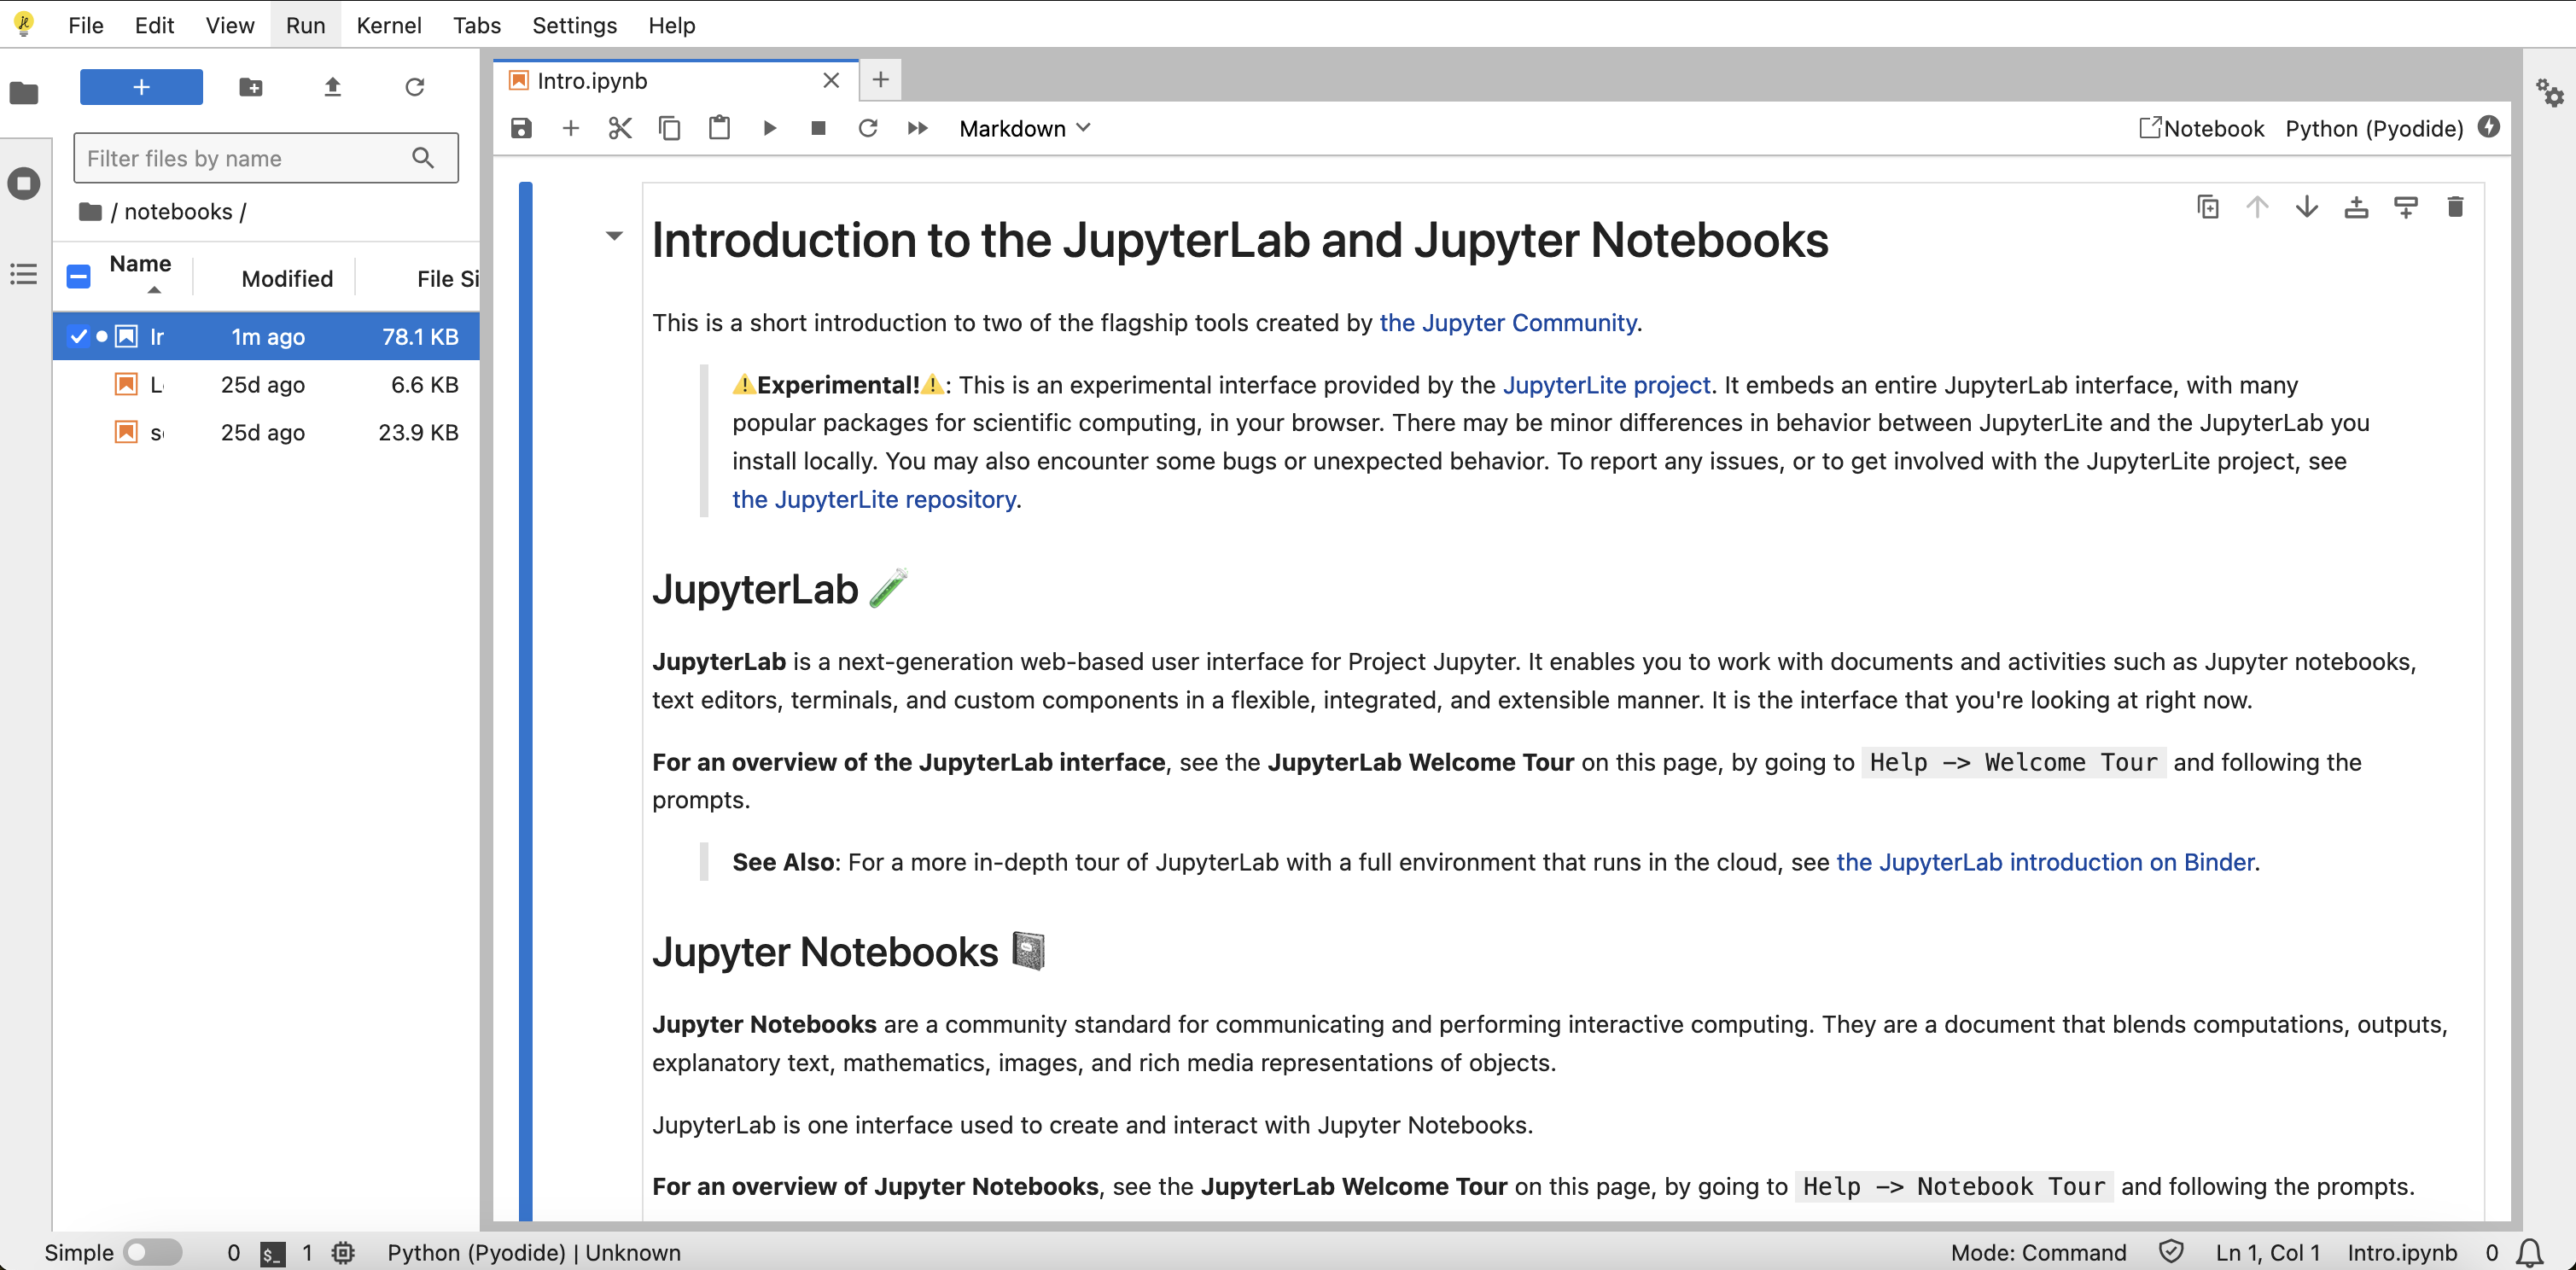
\includegraphics[width=0.75\textwidth]{images/jupyter-hub-1.png}
    \caption{Interfaccia di JupyterLab}
    \label{fig:jupyter-interface-1}
\end{figure}
\newline
JupyterLab si pone l'obiettivo di essere la piattaforma \textit{all-in-one} che permette di utilizzare in maniera più semplice l'ambiente precedente (Jupyter Notebook): l'interfaccia, visibile in figura \ref{fig:jupyter-interface-1}, è la stessa, infatti. 
\subsection{Funzionalità base di JupyterLab}
\subsubsection{Kernel Jupyter}
I kernel Jupyter\footnote{https://docs.jupyter.org/en/latest/projects/kernels.html} non sono altro che l'implementazione dei linguaggi di programmazione che possono essere utilizzati all'interno di un Jupyter Notebook, rendendo questo genere di ambienti estremamente estensibili. A rafforzare l'estensibilità di Jupyter, vi è il fatto che il framework utilizzato per implementare kernel, Xeus\footnote{https://xeus.readthedocs.io/en/latest/}, sia completamente \textit{open source}, rendendo, di fatto, realizzabili kernel per qualsiasi linguaggio di programmazione. Proprio per questo motivo, JupyterLab può vantare di una lunga lista di kernel disponibili\footnote{https://github.com/jupyter/jupyter/wiki/Jupyter-kernels}, tra i quali figurano Python, MatLab, Wolfram Mathematica, Gnuplot e molti altri.
\newline
È importante notare come i kernel Jupyter più popolari sono quelli dei linguaggi più usati in ricerca\cite{kluyver2016jupyter}: R e Python
\subsubsection{Creazione di un notebook}
Tramite la demo disponibile sul sito ufficiale\footnote{https://jupyter.org/try-jupyter/lab/}, è possibile interagire con un ambiente JupyterHub pre-impostato.
\newline
Per creare un notebook, basterà premere sul pulsante blu in alto a sinistra e selezionare l'ambiente Python per i notebook, come si può vedere in figura \ref{fig:jupyter-interface-2}.
\begin{figure}[h]
    \centering
    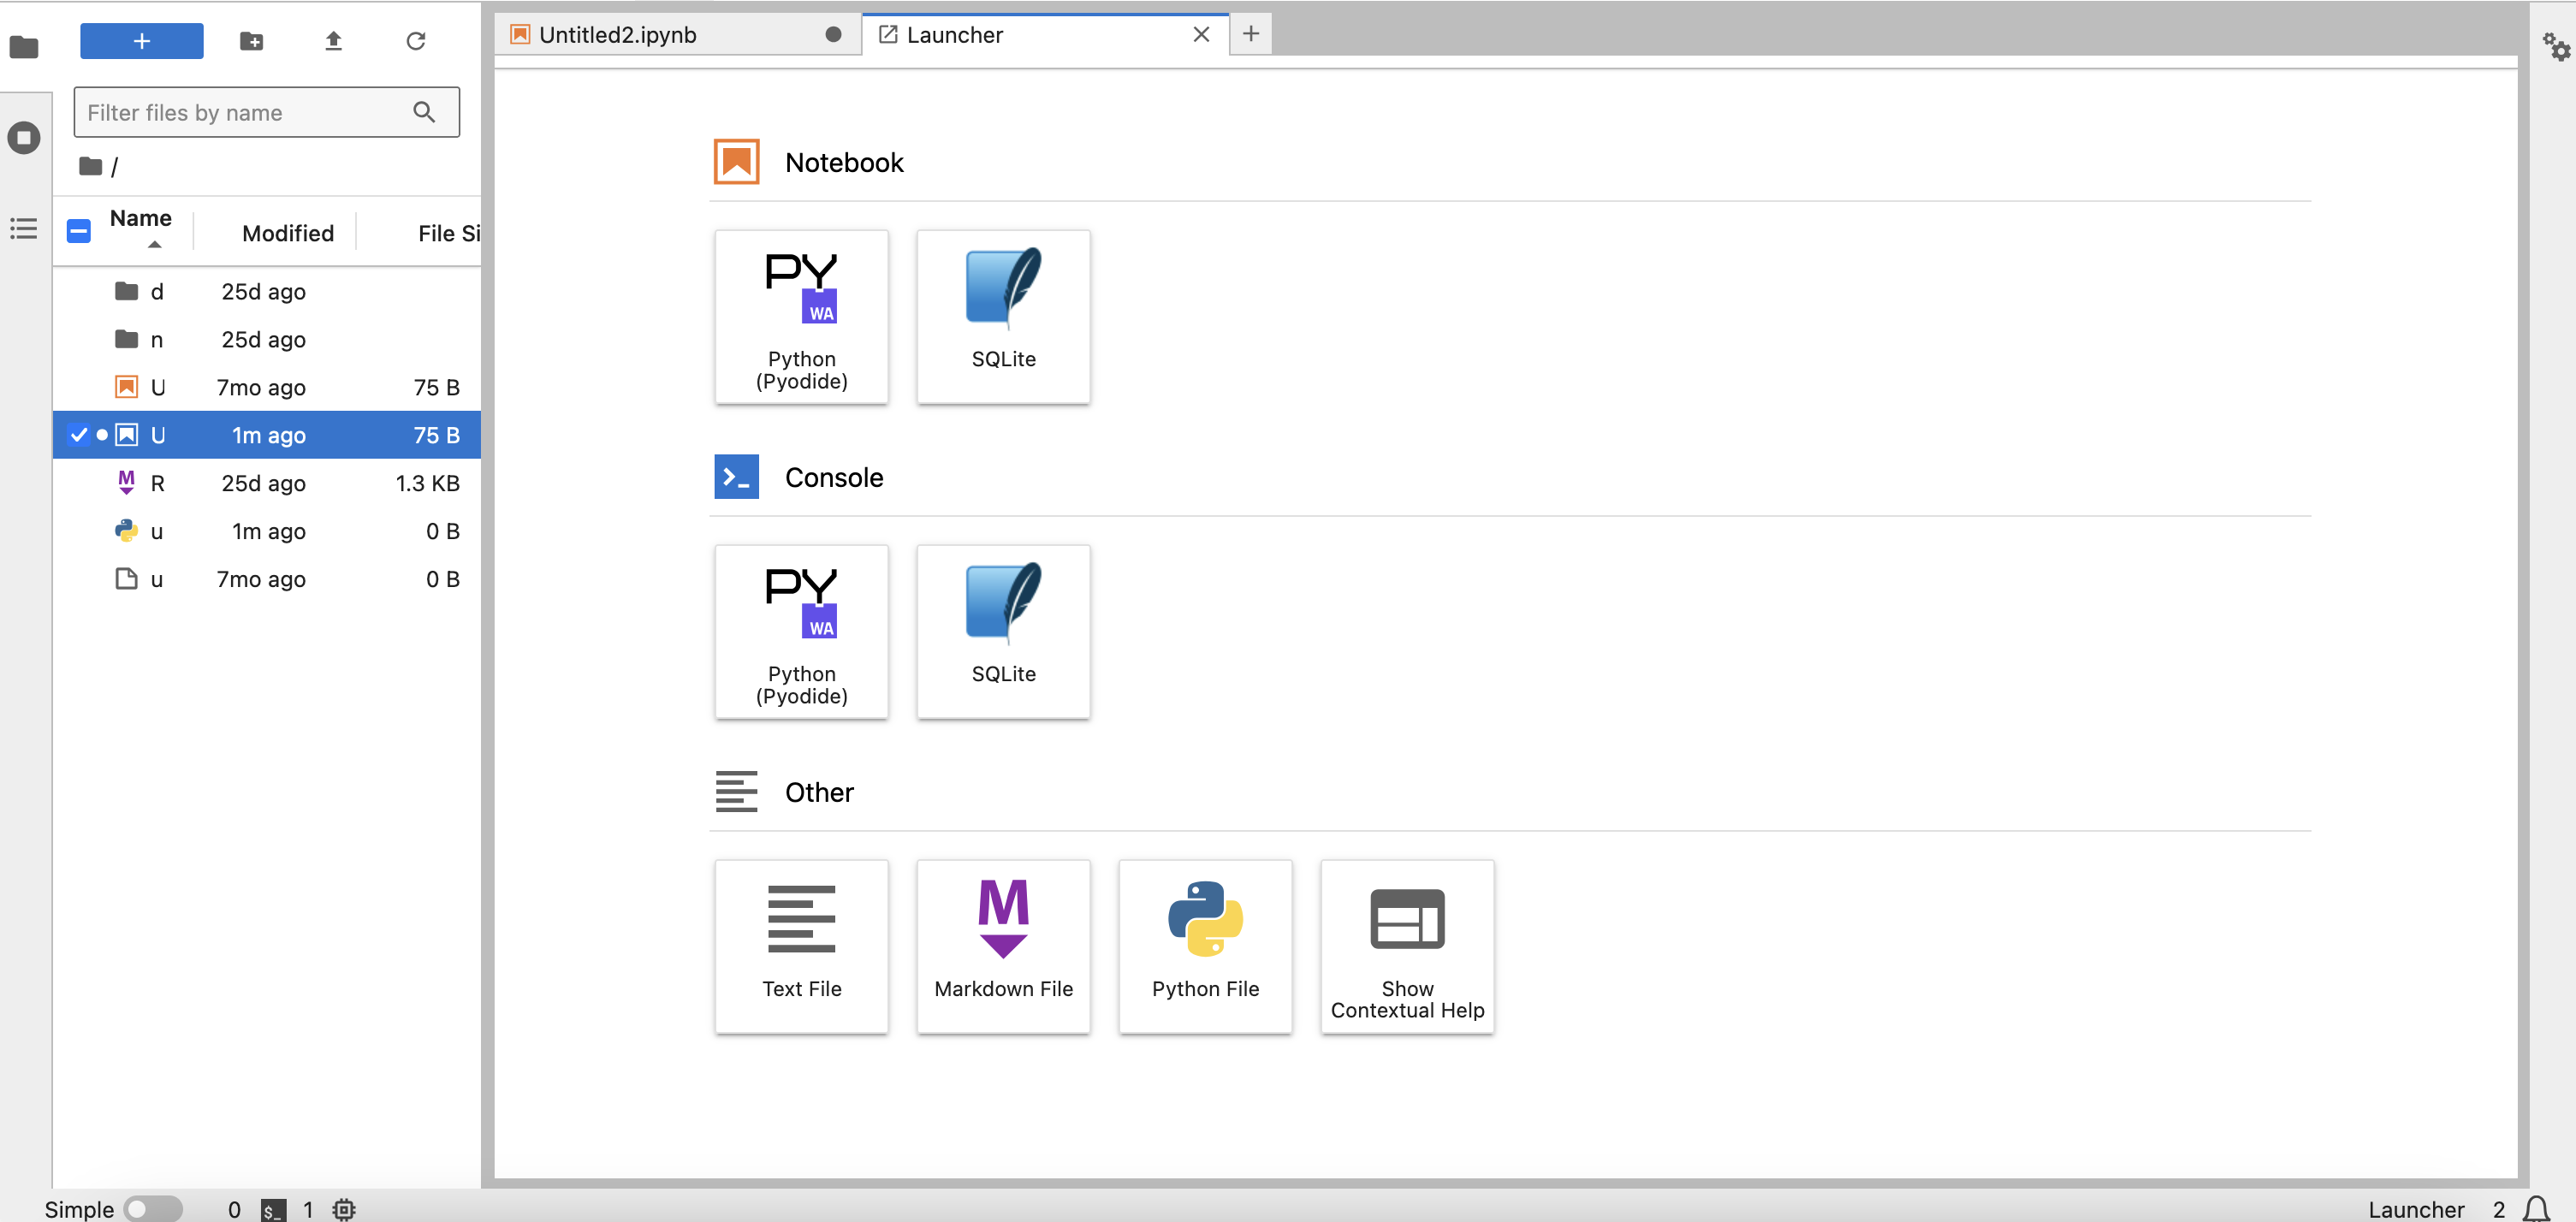
\includegraphics[width=0.75\textwidth]{images/jupyter-hub-2.png}
    \caption{Creazione di un notebook Python}
    \label{fig:jupyter-interface-2}
\end{figure}
\newline
Una volta creato il notebook, è possibile eseguire codice Python arbitrario al suo interno (figura \ref{fig:jupyter-interface-3}).
\begin{figure}[h]
    \centering
    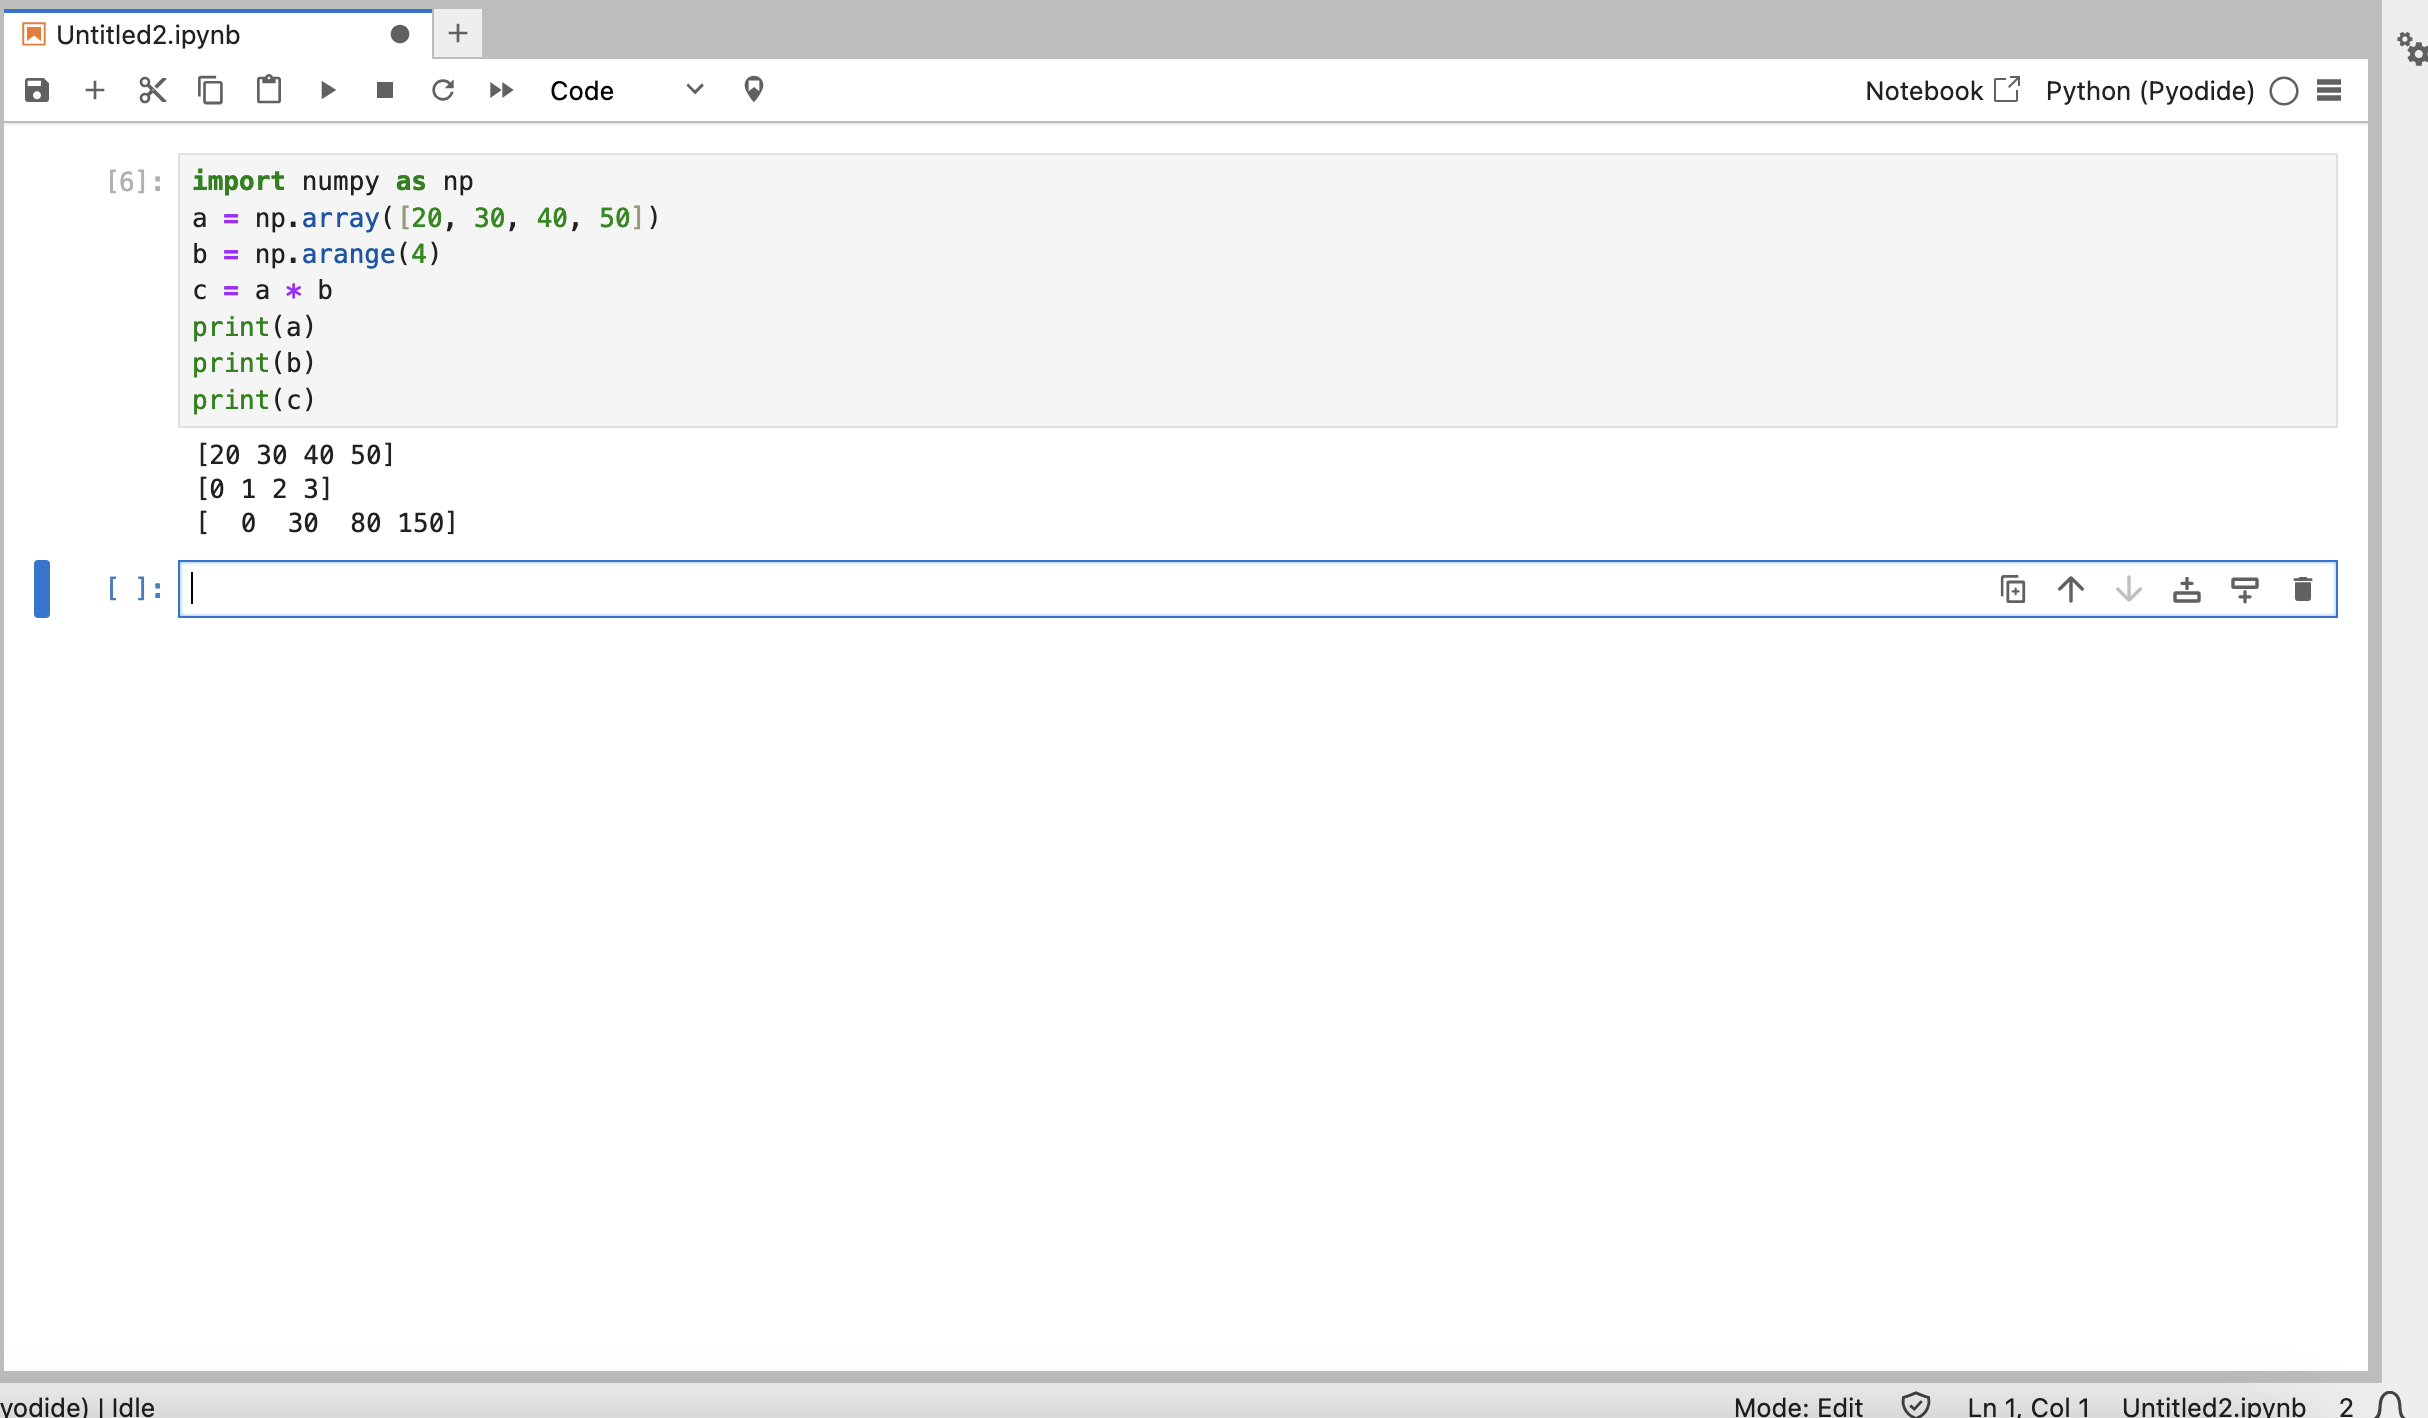
\includegraphics[width=0.75\textwidth]{images/jupyter-hub-3.png}
    \caption{Esecuzione codice Python in un notebook}
    \label{fig:jupyter-interface-3}
\end{figure}
\newpage
\section{Condivisione file}
È naturale che gruppi di ricerca, numerosi o meno che siano, necessitino di piattaforme su cui condividere e scambiare file in maniera veloce ed efficiente. L'accesso a questi file, poi, dovrà seguire un sistema di permessi, che permetterà a utenti con determinati privilegi di poter accedere o meno ai file in questione.\newline
Una ricerca di particolare spicco \cite{bosman_2016_49583}, che include più di ventimila risultati nel settore accademico, dimostra che servizi di condivisione file come Google Drive, che, in particolare, spicca per utilizzo, sono largamente adottati. Piattaforme di condivisione file come \textit{Google Drive}\footnote{https://drive.google.com} soddisfano sicuramente questo genere di requisiti, ma potrebbero non essere particolarmente adatte all'ambito accademico, principalmente per questioni riguardanti gli elevati costi di \textit{storage} e la privacy dei dati.
\newline
Sovente, infatti, le università scelgono di implementare \textit{in house} il proprio sistema di archiviazione e dematerializzazione dati, proprio per sopperire ai problemi succitati. Per questo motivo, l'utilizzo di piattaforme \textit{self-hosted} può sicuramente rappresentare una via percorribile per la gestione dei file senza ricorrere all'utilizzo di software commerciali gestiti esternamente.

\section{Nextcloud}
Nextcloud\footnote{https://nextcloud.com/} è una piattaforma \textit{open source} per la sincronizzazione e la condivisione di file, progettata per fornire un'alternativa autonoma ai servizi di cloud storage gestiti da terze parti. L'interfaccia utente è assolutamente familiare, anche ai più digiuni di informatica, rendendo l'esperienza utente e l'\textit{onboarding} di nuovi utenti particolarmente semplice.

\subsection{Sviluppo di applicazioni {ad-hoc} per Nextcloud}
È possibile sviluppare, in \textit{PHP}, apposite applicazioni che si possono integrare direttamente con la propria installazione di Nextcloud, un ulteriore punto a favore per l'utilizzo di questo software in ambito accademico.
\newline
È infatti molto probabile che un'istituzione come un'università abbia un portale di accesso con credenziali unificate, abbia bisogno di supporti personalizzati per processi interni e molto altro, rendendo la scelta di una piattaforma altamente personalizzabile come Nextcloud una necessità non negoziabile. 

\newpage
\section{Sfide}
Sebbene le tecnologie succitate siano estremamente versatili e di facile utilizzo, non si può dire altrettanto della loro installazione e manutenzione. Serve adibire personale alla gestione dello spazio virtuale per i documenti, a partire dalla configurazione dei \textit{server} sui quali i documenti fisicamente risiederanno, della rete che collega tali server, fino ad arrivare all'installazione dei vari servizi e l'esposizione di questi ultimi al pubblico.\newline
Oltre a ciò, uno dei problemi principali evidenziati dalla comunità scientifica riguarda la collaborazione e la condivisione dei risultati \cite{je2021reactive}.
\newline
Altri problemi, invece, derivano dal mero funzionamento del sistema, che dovrà fornire un grado di disponibilità (in termini di \textit{uptime}) generalmente alto, pertanto dovranno essere applicate logiche di replicazione e ridondanza che permettano un veloce recupero della stabilità del sistema nel caso di problemi dovuti a malfunzionamenti o interruzioni di servizio.
\newline
Queste sono le sfide che una piattaforma come \textit{NextPyter} si prefigge come obiettivi, per rendere la ricerca collaborativa quanto più accessibile possibile, sviluppando una soluzione che unisca la versatilità di JupyterLab alla familiarità e estensibilità di Nextcloud.